248. Муравьишка соревновался с улиткой в беге на 20 см. Когда муравьишка прибежал к финишу, улитке оставалось до него ещё 15 см. На сколько сантиметров надо отодвинуть назад стартовую линию для муравьишки, чтобы к финишу они приходили одновременно?\newpage
\noindent249. \begin{center}
\begin{figure}[ht!]
\center{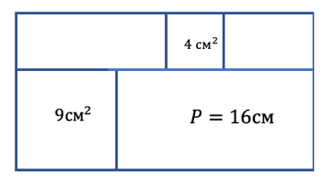
\includegraphics[scale=0.5]{kvadr.png}}
\end{figure}
\end{center}
Вася вырезал из бумаги два квадрата и три прямоугольника, а затем сложил из них большой прямоугольник (см. рисунок). Найдите площадь  полученного Васей прямоугольника, если площади квадратов равны $4\text{ см}^2$ и $9\text{ см}^2,$ а периметр одного из прямоугольников --- 16 см.\\
